\chapter{Методы восстановления трехмерных моделей}

В данной главе рассматриваются различные подходы к восстановлению трехмерных
моделей по двумерным изображениям. Исследование начинается с анализа
классического подхода, основанного на методах структуры из движения (Structure
from Motion) и многовидовой стереоскопии (Multi-View Stereo), не использующего
нейросетевые технологии. Затем рассматриваются два современных нейросетевых
метода: первый основан на архитектуре \textit{TensoRF}, а второй использует
\textit{<BLANK>}. Сравнение этих подходов позволяет выявить преимущества и
ограничения применения нейросетевых технологий в задачах трехмерной
реконструкции.

Все эксперименты выполнялось на облачном экземпляре OpenStack Nova (Selectel) с
ОС Ubuntu 22.04 LTS: 2 x Intel Xeon Silver 4214R @ 2,4 ГГц (8 физических ядер),
16 ГиБ ОЗУ, GPU NVIDIA Tesla T4 с 16 ГиБ памяти и SSD-томом 100 ГиБ. Приложение
\texttt{COLMAP} было собрано из исходников версии 3.11.1 с настройками
\texttt{GUI\_ENABLED=OFF}, \texttt{CUDA\_ENABLED=ON},
\texttt{CMAKE\_CUDA\_ARCHITECTURES=75}.

\section{Классический фотограмметрический подход}

В качестве точки отсчета мы используем открытый пакет
\texttt{COLMAP} \cite{10.1109/CVPR.2016.4454}. С точки зрения
пользователя \texttt{COLMAP} реализует двухэтапный конвейер обработки изображений
(англ. \emph{pipeline}):

\begin{enumerate}
  \item \textbf{Structure-from-Motion (SfM)} решает задачу одновременного восстановления \emph{(i)} трёхмерной структуры
  сцены и \emph{(ii)} внутренних ($K$) и внешних ($R,t$) параметров всех камер.
  На практике процесс разбивается на три минимальные стадии:

  \begin{enumerate}
    \item \emph{Поиск и описание особенностей изображения} — детектирование
    характерных точек (например, \textsc{SIFT} \cite{lowe2004distinctiveimagefeatures}), формирование их дескрипторов.
    \item \emph{Сопоставление и геометрическая проверка} — построение парных
    соответствий между изображениями и отбраковка ложных совпадений с помощью
    алгоритма RANSAC (англ.\ \emph{Random Sample Consensus}).
    \item \emph{Совместная реконструкция структуры и движения} —
     одновременная оценка 3D координат точек и параметров всех камер через
     Bundle Adjustment, минимизирующий суммарную пере‑проекционную ошибку.
  \end{enumerate}

  Результатом этапа SfM служит разреженное облако точек сцены, а также
  восстановленные матрица внутренних параметров $K$ и позы камер $(R,t)$,
  которые впоследствии можно использовать как входные данные для более поздних
  (в том числе нейросетевых) этапов плотной реконструкции.

  \item \textbf{Multi-View Stereo (MVS)} начинается с результатов SfM и
  преобразует их в плотную геометрию сцены. Процесс обычно делят на три
  стадии:

  \begin{enumerate}
    \item \emph{Оценка карты глубин и нормалей для каждого кадра} — алгоритмы
    семейства PatchMatch-Stereo определяют для каждой пиксельной проекции
    предполагаемое расстояние до сцены и ориентацию её локальной поверхности.
    \item \emph{Слияние (``fusion'') карт глубин} — данные нескольких
    перекрывающихся изображений преобразуются в общее плотное облако точек, где
    каждой точке сопоставлена усреднённая глубина и нормаль.
    \item \emph{Восстановление сплошной поверхности} не составляет труда, когда
    плотное облако точек и нормали уже вычислены. На практике чаще всего
    применяют пуассоновскую\footnote{Симеон Дени Пуассон (фр. Simeon Denis
    Poisson; 21 июня 1781, Питивье, Франция — 25 апреля 1840, Со, Франция) —
    французский математик, механик и физик.} реконструкцию поверхности
    \cite{10.1145/2487228.2487237} либо триангуляцию Делоне\footnote{Борис
    Николаевич Делоне (3 марта 1890, Санкт-Петербург — 17 июля 1980,
    Москва) — русский и советский математик, профессор МГУ, член-корреспондент
    АН СССР.} с последующей фильтрацией.
  \end{enumerate}

  На выходе этапа MVS получается высокодетализированная
  плотная модель (точечное облако или треугольная сетка), которая
  может служить финальным результатом либо исходными данными для
  дальнейшей обработки.
\end{enumerate}

\noindent Обе стадии опираются исключительно на классические методы эпиполярной геометрии
и вариационного анализа; никаких нейросетевых компонентов здесь нет.

Во всех опытах применялись синтетические наборы изображений, сформированные
скриптом \texttt{generate-batch}. В данном разделе датасет содержит 200
кадров размером $224\times224$~px; центры виртуальных камер расположены по
кольцевой траектории верхней полусферы с полярным углом $\theta = 0.7\frac{\pi}{2}$.

\begin{figure}[h]
    \centering
    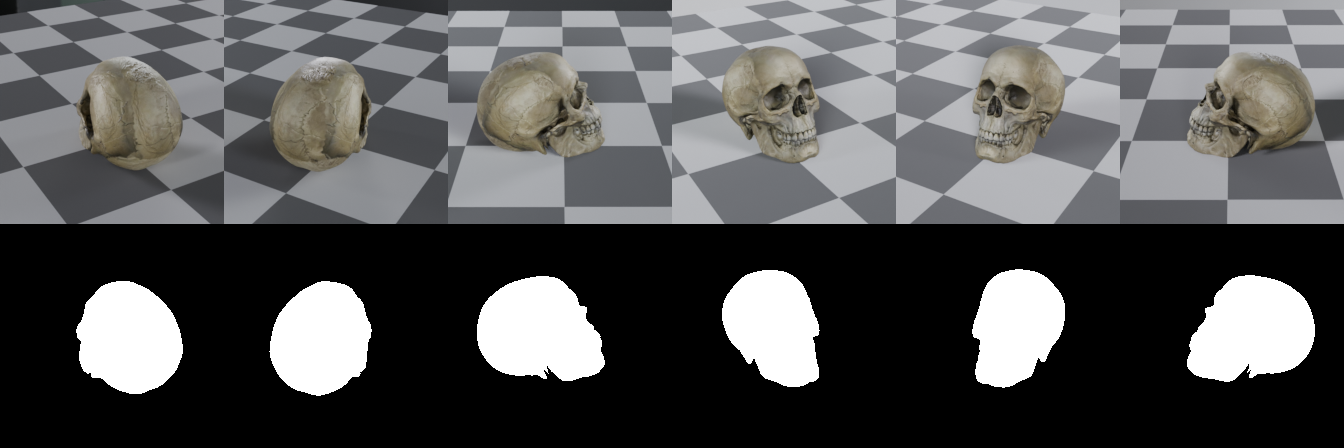
\includegraphics[width=0.8\textwidth]{skull-male-preview.png}
    \caption{Сцена 1}
    \label{fig:scene1}
\end{figure}

Рассмотрено четыре варианта настроек \texttt{COLMAP}, отличающихся уровнем
качества, использованием бинарных масок и наличием априорной калибровки камер.

\subsection{Эксперимент 0: \texttt{automatic\_reconstruction}}

Без масок и при стандартных настройках SfM уверенно восстанавливает все 200
позиций камер (рис.~\ref{fig:0sparse}), но MVS улавливает не только череп, но и
шахматный пол, образуя характерный «ковёр» из точек (рис.~\ref{fig:0fusion}).
Пустоты на верхней части модели и распыление фона наводят на мысль, что
алгоритму мешает низко‑текстурированная плоскость. Попробуем использовать маски,
чтобы ``спрятать'' фон.

% Картинки с Fusion были открыты в blender и отрендерерны как вьюпорт
% с предварительной обработкой: цвет вьюпорта изменен на белый, объекты выровнены по осям
% и в геометрии была добавлена нода "Mesh to Points", чтобы точки выглядели жирнее
\begin{figure}[h]
    \centering
    \begin{subfigure}[b]{0.3\textwidth}
        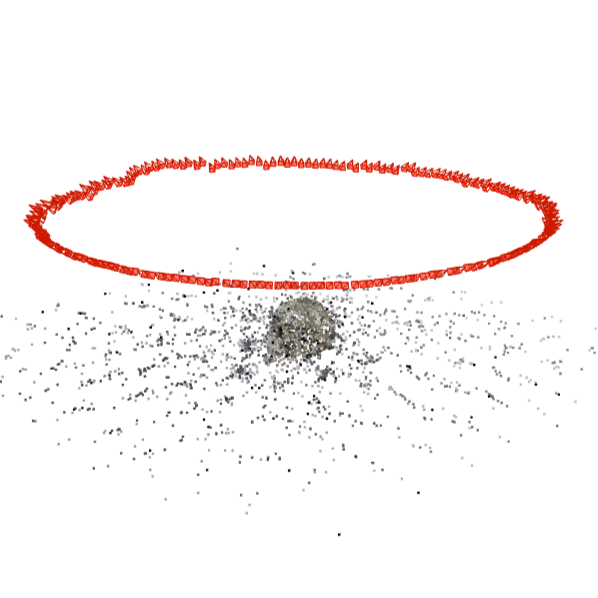
\includegraphics[width=\textwidth]{0-sparse.png}
        \caption{Sparse}
        \label{fig:0sparse}
    \end{subfigure}
    \hfill
    \begin{subfigure}[b]{0.3\textwidth}
        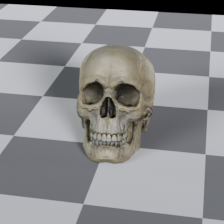
\includegraphics[width=\textwidth]{0-undistorted.png}
        \caption{Undistorted}
        \label{fig:0undistorted}
    \end{subfigure}
    \hfill
    \begin{subfigure}[b]{0.3\textwidth}
        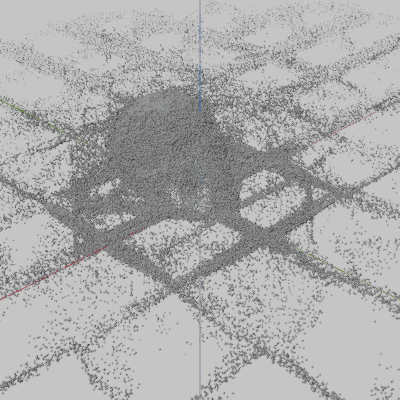
\includegraphics[width=\textwidth]{0-fusion.png}
        \caption{Fusion}
        \label{fig:0fusion}
    \end{subfigure}
    \caption{Эксперимент 0}
    \label{fig:0exp}
\end{figure}

\subsection{Эксперимент 1: \texttt{automatic\_reconstruction} + маски}

Маскирование действительно устраняет шум пола:
облако точек стало компактнее и чище
(рис.~\ref{fig:1fusion}). Однако вместе с фоном
исчезла большая чсть ключевых точек, и SfM реконструирует
лишь часть кольца камер (рис.~\ref{fig:1sparse}),
а некоторые мелкие детали черепа сглажены. Попробуем изменить настройки:
увеличить глубину поиска и число итераций, чтобы компенсировать потерю особенностей.

\begin{figure}[h]
    \centering
    \begin{subfigure}[b]{0.3\textwidth}
        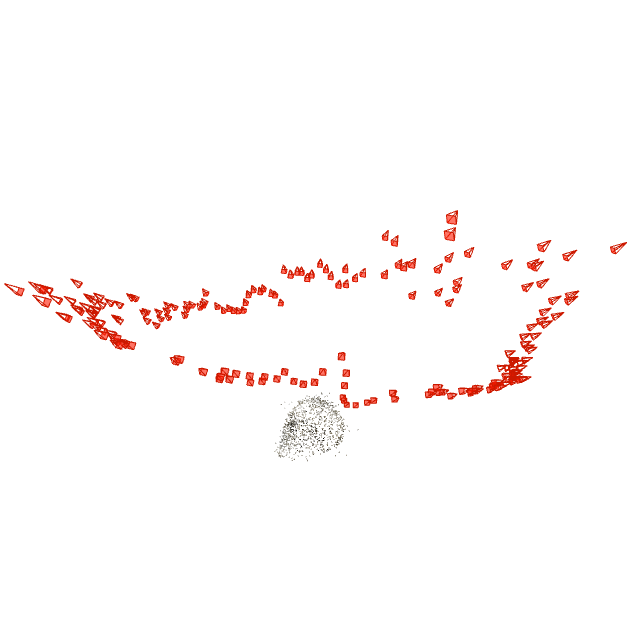
\includegraphics[width=\textwidth]{1-sparse.png}
        \caption{Sparse}
        \label{fig:1sparse}
    \end{subfigure}
    \hfill
    \begin{subfigure}[b]{0.3\textwidth}
        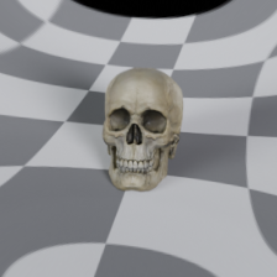
\includegraphics[width=\textwidth]{1-undistorted.png}
        \caption{Undistorted}
        \label{fig:1undistorted}
    \end{subfigure}
    \hfill
    \begin{subfigure}[b]{0.3\textwidth}
        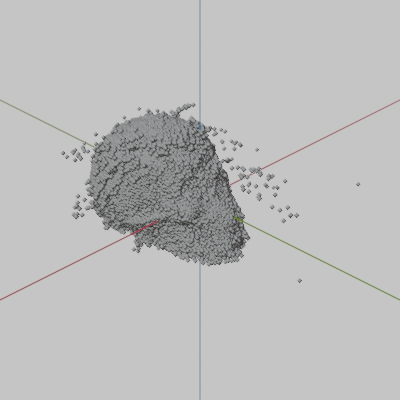
\includegraphics[width=\textwidth]{1-fusion.png}
        \caption{Fusion}
        \label{fig:1fusion}
    \end{subfigure}
    \caption{Эксперимент 1}
    \label{fig:1exp}
\end{figure}

\subsection{Эксперимент 2: \texttt{extreme} \texttt{automatic\_reconstruction} + маски}

Более агрессивные параметры возвращают почти все камеры
(рис.~\ref{fig:2sparse}), но оптимизатор ошибочно
объясняет различия в масках сильной радиальной дисторсией,
что хорошо видно по деформированному узору пола
(рис.~\ref{fig:2undistorted}). В результате
плотная модель окружена выбросами (рис.~\ref{fig:2fusion}).
Попробуем зафиксировать калибровку и позы камер
до запуска COLMAP, чтобы снять двусмысленность.

\begin{figure}[h]
    \centering
    \begin{subfigure}[b]{0.3\textwidth}
        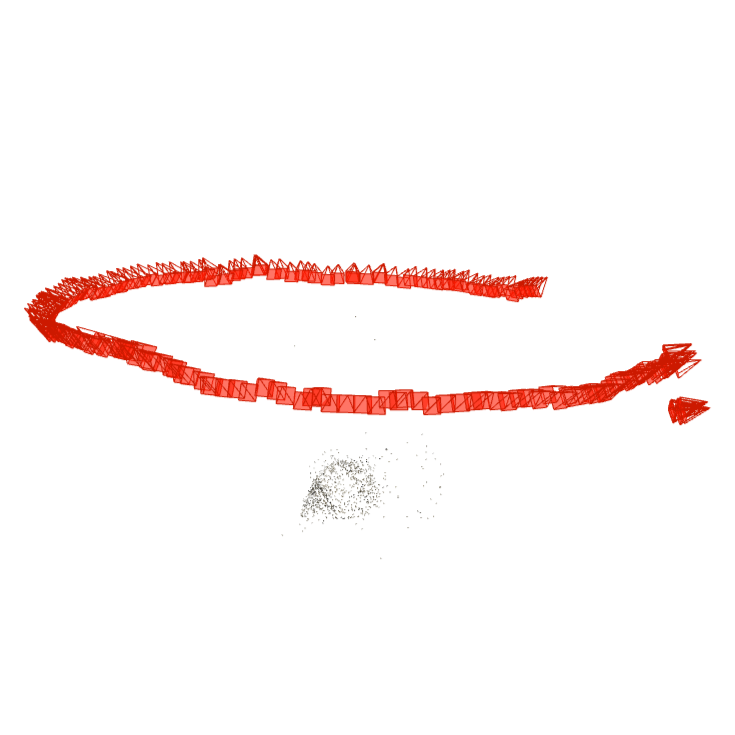
\includegraphics[width=\textwidth]{2-sparse.png}
        \caption{Sparse}
        \label{fig:2sparse}
    \end{subfigure}
    \hfill
    \begin{subfigure}[b]{0.3\textwidth}
        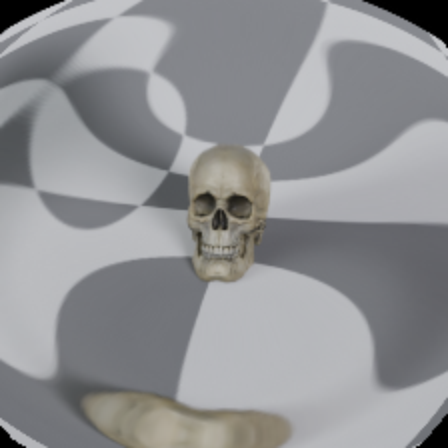
\includegraphics[width=\textwidth]{2-undistorted.png}
        \caption{Undistorted}
        \label{fig:2undistorted}
    \end{subfigure}
    \hfill
    \begin{subfigure}[b]{0.3\textwidth}
        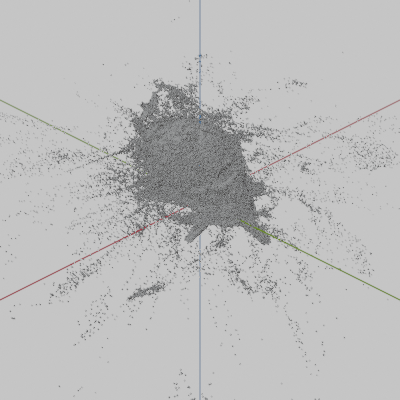
\includegraphics[width=\textwidth]{2-fusion.png}
        \caption{Fusion}
        \label{fig:2fusion}
    \end{subfigure}
    \caption{Эксперимент 2}
    \label{fig:2exp}
\end{figure}

\subsection{Эксперимент 3: априорные позы + маски, качество \texttt{extreme}}

С помощью скрипта \texttt{generate-batch} и плагинов
\texttt{camera\_extrinsics} и \texttt{camera\_intrinsics} были получены внешние
и внутренние параметры камеры Blender. Предложенный в рамках этой работы скрипт
\texttt{to\_colmap}\footnote{Исходный код и примеры использования можно найти по
постоянной ссылке
\url{https://github.com/SherAndrei/blender-gen-dataset/tree/0a8cd30e94b21ec3442b2c315cf05be47b3b214c/scripts/to_colmap}}
позволяет заранее задать внешние и внутренние параметры камер в \texttt{COLMAP}
проекте (\texttt{cameras.txt}, \texttt{images.txt}, \texttt{database.db}), тем
самым позволяя полностью пропустить шаг с SfM.

MVS смог обеспечить наиболее плотную реконструкцию среди всех опытов
(рис.~\ref{fig:3fusion}): лобная и носовая части черепа воспроизводятся с
минимумом пропусков. Тем не менее боковые поверхности и задняя часть черепа
страдают от зеркальных бликов — в этих областях MVS по‑прежнему создаёт выбросы
и пропуски.

\begin{figure}[h]
    \centering
    \begin{subfigure}[b]{0.3\textwidth}
        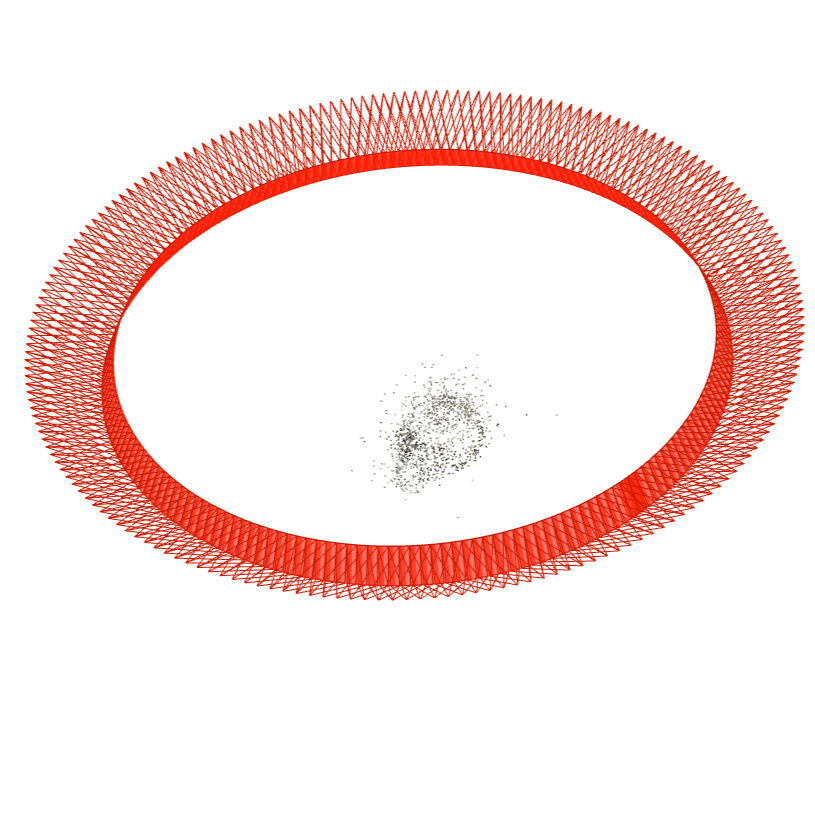
\includegraphics[width=\textwidth]{3-sparse.png}
        \caption{Sparse}
        \label{fig:3sparse}
    \end{subfigure}
    \hfill
    \begin{subfigure}[b]{0.3\textwidth}
        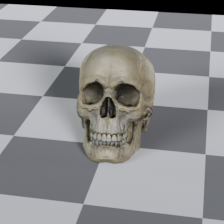
\includegraphics[width=\textwidth]{3-undistorted.png}
        \caption{Undistorted}
        \label{fig:3undistorted}
    \end{subfigure}
    \hfill
    \begin{subfigure}[b]{0.3\textwidth}
        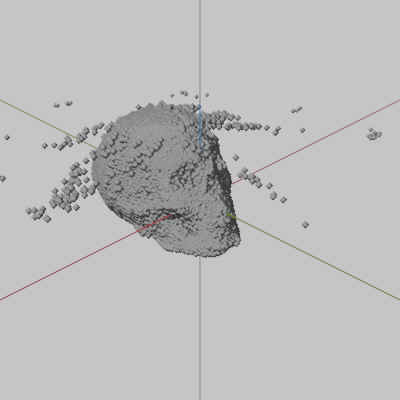
\includegraphics[width=\textwidth]{3-fusion.png}
        \caption{Fusion}
        \label{fig:3fusion}
    \end{subfigure}
    \caption{Эксперимент 3}
    \label{fig:3exp}
\end{figure}

\subsection{Эксперимент 4: Использование реальных данных}

Для проверки устойчивости классического конвейера на практическом материале был
взят видеоролик длиной 26 секунд, снятый на смартфон Samsung Galaxy A52.
Камера оставалась неподвижной, а небольшая фигурка слона из папье‑маше вращалась
на круглом пьедестале, благодаря чему получилась имитация кругового облёта
объекта. Из видеопоследовательности были извлечены сто восемьдесят восемь кадров
с частотой семь кадров в секунду с помощью программы \texttt{ffmpeg}; параметры
сжатия и оригинальное разрешение сохранены без изменений, см. рис. \ref{fig:elephant-preview}.

\begin{figure}[h]
  \centering
  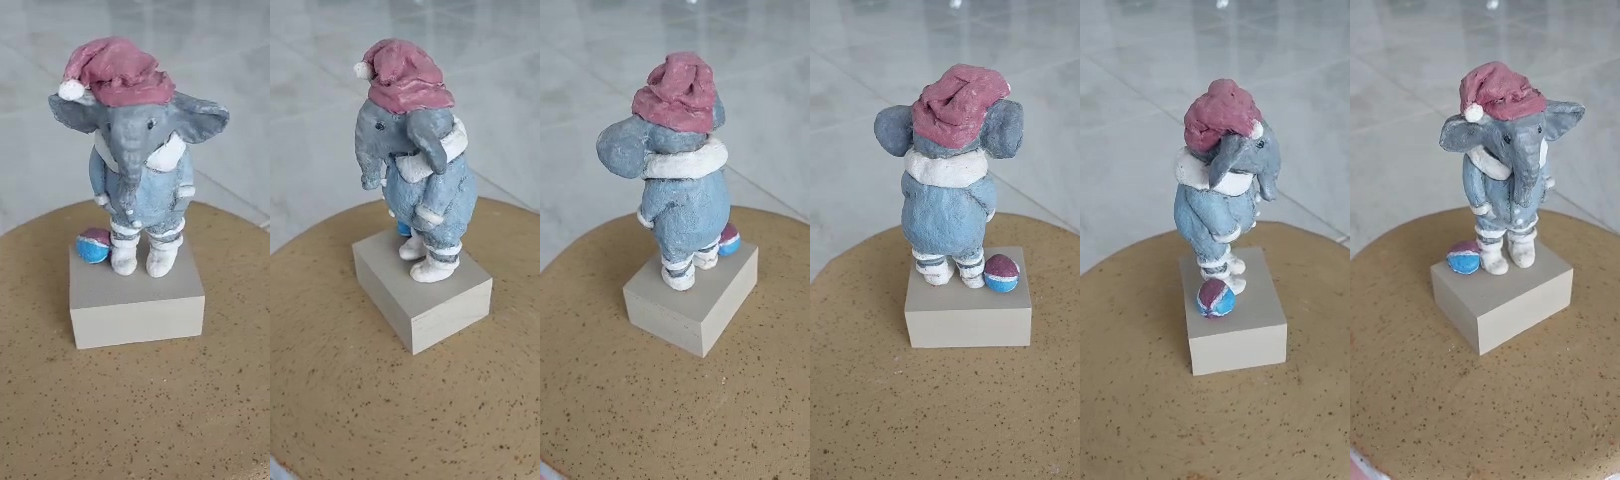
\includegraphics[width=\textwidth]{elephant-preview.png}
  \caption{Датасет фигуры из папье-маше}
	\label{fig:elephant-preview}
\end{figure}

Обработка выполнялась в \texttt{COLMAP} с использованием
\texttt{automatic\_reconstruction} с уровнем качества \texttt{extreme}. В
качестве оптимизации задействован \texttt{sequential\_matcher}, а также
указано использование единственной камеры. Полный
цикл «SfM + MVS» занял чуть больше 32 двух минут на рабочей станции.

\begin{figure}[h]
    \centering
    \begin{subfigure}[b]{0.3\textwidth}
        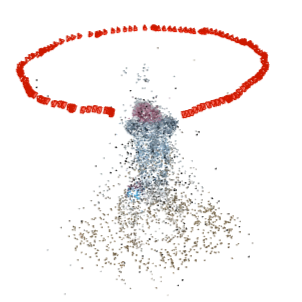
\includegraphics[width=\textwidth]{4-sparse.png}
        \caption{Sparse}
        \label{fig:4sparse}
    \end{subfigure}
    \begin{subfigure}[b]{0.3\textwidth}
        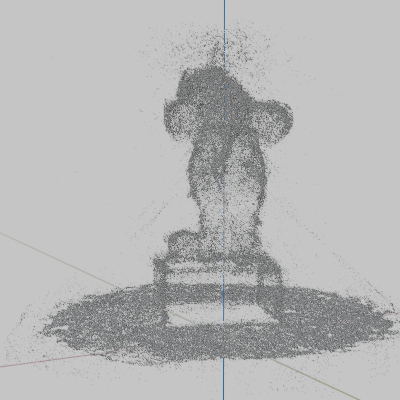
\includegraphics[width=\textwidth]{4-fusion.png}
        \caption{Fusion}
        \label{fig:4fusion}
    \end{subfigure}
    \caption{Эксперимент 4}
    \label{fig:4exp}
\end{figure}

Полученная разреженная модель показала, что алгоритм и корректно восстановил
замкнутую траекторию камер, и определил положение фигурки без заметных
отклонений. Обилие текстурных элементов на отдалённом фоне дополнительно
стабилизировало процесс bundle adjustment и снизило вероятность вырождения
оптимизации. Плотное облако точек, полученное после этапа fusion, содержало
выраженную «корону» из шумовых точек по периметру модели. Этот артефакт был
вызван теми же фон‑специфичными признаками, которые помогали SfM, — при переходе
к MVS они оказались ошибочно привязанными к объекту интереса, см. \ref{fig:floor-as-feature}.

\begin{figure}[h]
    \centering
    \begin{subfigure}[b]{0.2\textwidth}
        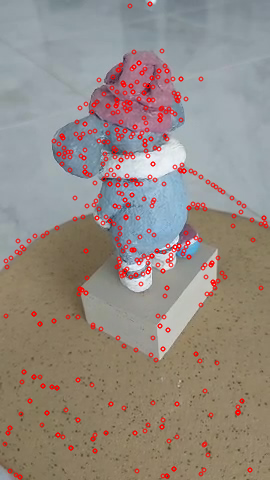
\includegraphics[width=\textwidth]{0-floor-as-feature.png}
    \end{subfigure}
    \begin{subfigure}[b]{0.2\textwidth}
        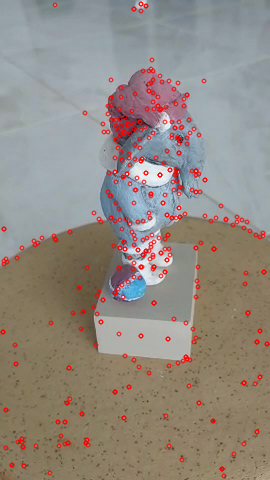
\includegraphics[width=\textwidth]{1-floor-as-feature.png}
    \end{subfigure}
    \caption{Пол считается частью объекта}
    \label{fig:floor-as-feature}
\end{figure}

Качество реконструкции оказалось сопоставимо с самым первым синтетическим
опытом: геометрия слона читается, однако детализация заметно ухудшена за счёт
шумов. Основной вывод заключается в том, что даже при съёмке на обычный смартфон
и при отсутствии строгого контроля за сценой классический алгоритм способен
обеспечить полноценную трёхмерную реконструкцию. При этом главной проблемой
остаётся борьба с фоновой информацией: либо сцену следует подготавливать, либо
необходимо применять очистку плотного облака.

\subsection{Выводы}

Разбор последовательных экспериментов позволяет выделить
устойчивые особенности работы классической связки SfM+MVS:

\begin{itemize}
    \item При богатой текстуре и отсутствии масок метод уверенно восстанавливает
    кольцевую траекторию камер и создаёт приемлемую плотность модели.

    \item Маскирование удаляет шум пола и делает облако чище, но одновременно
    обедняет граф соответствий; часть камер не восстанавливается, а мелкие
    детали сглаживаются.

    \item Изменение настроек алгоритмов компенсирует нехватку патчей,
    однако без жёсткой калибровки маски интерпретируются как радикальная
    дисторсия, что приводит к расплыванию геометрии.

    \item Предварительно зафиксированные интринзики и позы снимают
    неоднозначность и дают лучший баланс плотности и чистоты, однако зеркальные
    блики и самоокклюзии всё ещё рождают выбросы и пробелы — предел классической
    фотограмметрии.
\end{itemize}

\noindent Чтобы преодолеть ограничения классической фотограмметрии — зеркальные
блики, маски, скудную текстуру и самоокклюзии — необходима более выразительная
регуляризация. Именно её предлагают современные нейронные методы (NeRF, TensoRF
и др.). В следующей главе мы последовательно разберём эти архитектуры, покажем,
каким образом они используют параметры камер, полученные SfM, и сравним их
результаты с классическим подходом на тех же тестовых сценах.

\section{Тензорные поля излучения}

В 2020 году модель \emph{Neural Radiance Fields} (NeRF) впервые показала, что по
набору фотографий и поз камер можно восстановить непрерывную функцию, которая
для любой точки пространства возвращает плотность $\sigma$ и цвет $\mathbf{c}$.
Решение хранилось внутри большого MLP, обучавшегося днями на одну сцену и
требовавшего сотни мегабайт памяти.

Необходимость ускорить обучение и снизить потребление памяти
привела к идее компактных представлений.
Ответом стал \emph{TensoRF} (2022):
он сохраняет саму формулировку задачи NeRF: «какой цвет и какая плотность
в каждой точке?», но заменяет тяжёлый MLP на низкоранговую
\emph{тензорную факторизацию} радианс‑поля.

Вместо полного 3D массива $D_x\times D_y\times D_z$ TensoRF хранит три набора
«полосок» вдоль осей $X$, $Y$, $Z$.  Память падает с $\mathcal{O}(D^3)$ до
$\mathcal{O}(3RD)$, где $R$ — ранг разложения. Из‑за малого числа параметров
(обычно $\sim10^6$ против $\sim10^8$ у NeRF) обучение одной сцены занимает
десятки минут на GPU.

TensoRF ``подхватил'' идею NeRF описывать сцену непрерывной функцией, но
переформулировал хранение этой функции как низкоранговую таблицу умножения
одномерных векторов.  В результате добился сопоставимого качества при
существенно меньших вычислительных и временных затратах.

Для оценки реальных возможностей TensoRF мы провели
четыре последовательных эксперимента\footnote{Код
и конфигурационные файлы доступны в репозитории проекта по ссылке \url{https://github.com/SherAndrei/3d-reconstruction}.}.
Результат работы модели оценивается с помощью метрики PSNR (англ. \emph{Peak signal-to-noise ratio}),
чем выше результат которой, тем лучше, приемлемыми считаются значения больше 30 дБ.

\subsection{Эксперимент 0: Диффузный объект}
Сцена — уже известная 3D модель черепа; датасет из 200 фотографий, сгенерированных скриптом
\texttt{generate-batch} с масками, заранее задами позами и внутренними
параметрами камер. Разбиение: 150 кадров в train, 50 в test.  Обучение на GPU
Tesla T4 заняло $10$ минут; получена средняя $\operatorname{PSNR} = 44.26$ дБ.

\begin{figure}[h]
  \centering
  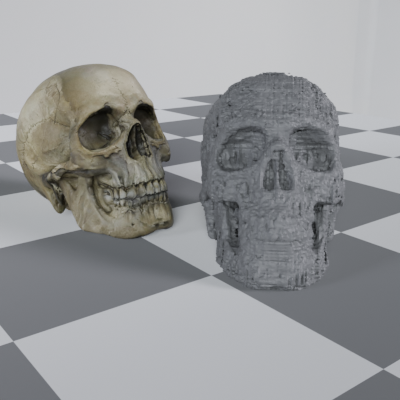
\includegraphics[width=0.3\textwidth]{tensorf-skull.png}
  \caption{Восстановленная модель черепа рядом с оригинальной}
\end{figure}

\subsection{Эксперимент 1: Драгоценный камень в макросъёмке}
Аналогичный набор с заранее известными позами камер из 200 кадров размера
$400\times400$~px представлен на рис.  \ref{fig:asscher-preview}, Сцену
составляет прозрачный огранённый камень в сравнимых с реальным драгоценным
камнем в размерах, из-за чего съёмка виртуальной камерой производится с большим
фокусным расстоянием (камень занимает почти весь кадр).

\begin{figure}[h]
  \centering
  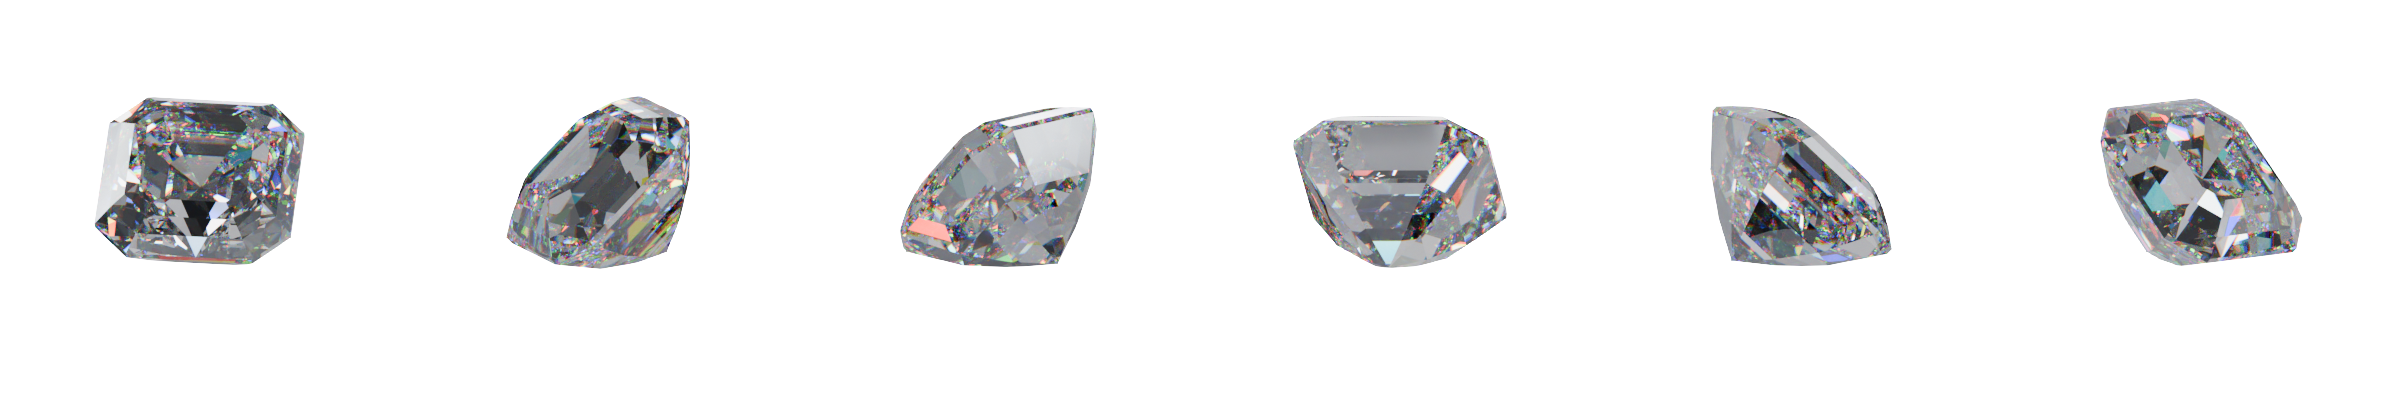
\includegraphics[width=0.8\textwidth]{diamond-asscher-masked-preview.png}
  \caption{Используемый датасет драгоценного камня}
	\label{fig:asscher-preview}
\end{figure}

TensoRF выдал заметно худший результат $\operatorname{PSNR}=23.13$ дБ; на
рис.~\ref{fig:tensorf-asscher-small} видно искажение — модель не распознала
реальный микроскопический масштаб и сформировала лишь размытый объём с шумом.

\subsection{Эксперимент 2: «Обман масштаба».}
Чтобы проверить гипотезу о влиянии масштаба сцены, с помощью
\texttt{generate-batch} были сгенерированы соответствующие позы и внутренние
параметры камер, совпадающие с параметрами, которые использовались для
черепа\footnote{Обращаю внимание, что так как размер изображения драгоценного
камня отличается от размера изображения черепа, то отличаются и внутренние
параметры у камер, поэтому генерацию нужно проделывать заново.}.
Новые параметры подложили в датасет с изображениями бриллианта.
При тех же настройках обучения удалось получить приемлемое качество, $\operatorname{PSNR}=29.17$
(cм. рис.~\ref{fig:tensorf-asscher-large}).


\begin{figure}[h]
    \centering
    \begin{subfigure}[h]{0.45\textwidth}
      \centering
      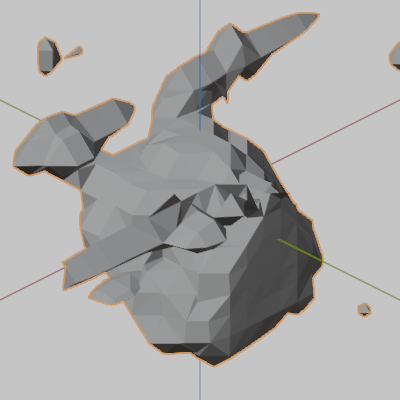
\includegraphics[width=0.6\textwidth]{tensorf-asscher-small.png}
      \caption{Неудачная попытка восстановления}
      \label{fig:tensorf-asscher-small}
    \end{subfigure}\hfill
    \begin{subfigure}[h]{0.45\textwidth}
     \centering
      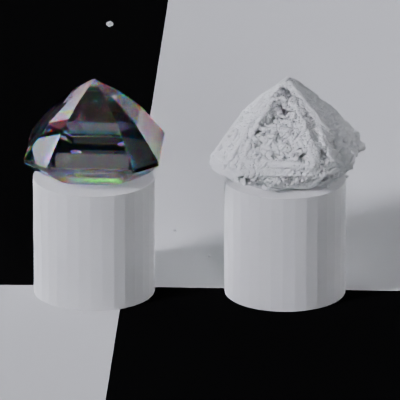
\includegraphics[width=0.6\textwidth]{tensorf-asscher-large.png}
      \caption{Восстановленный драгоценный камень}
      \label{fig:tensorf-asscher-large}
    \end{subfigure}
    \caption{}
\end{figure}

Тем не менее прозрачная структура
привела к локальным пустотам внутри тела,
что косвенно указывает на сложности модели
с реконструкцией стекло‑подобных материалов.

\subsection{Эксперимент 3: Использование реальных данных}

В качестве входных данных использовался тот же видеоролик с фигуркой
слонёнка, что и в соответствующем классическом эксперименте.
Датасет был разбит на две части: 141 кадр в трейн‑выборке
и 46 кадров в тестовой. Поскольку COLMAP ранее уже оценил
внешние и внутренние параметры камеры, эти калибровочные
данные были напрямую переиспользованы в процессе обучения TensoRF.

Главное отличие от синтетических примеров заключается в отсутствии
бинарных масок: TensoRF должен самостоятельно «догадаться»,
где заканчивается объект и начинается фон. По умолчанию
алгоритм ограничивает область поиска коробкой
$\verb|scene_bbox|$ с координатами от $(-1.5,-1.5,-1.5)$
до $(1.5,1.5,1.5)$. Однако фигурка вместе с пьедесталом в эти
границы не помещалась: часть модели обрезалась, что хорошо видно
на рис.~\ref{fig:tensorf_elephant_bad}.

\begin{figure}[h]
    \centering
    \begin{subfigure}[b]{0.45\textwidth}
        \centering
        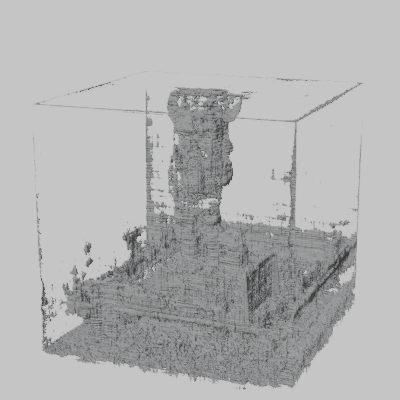
\includegraphics[width=0.6\textwidth]{tensorf-elephant-bad-bbox.png}
        \caption{До настройки параметров}
        \label{fig:tensorf_elephant_bad}
    \end{subfigure}\hfill
    \begin{subfigure}[b]{0.45\textwidth}
        \centering
        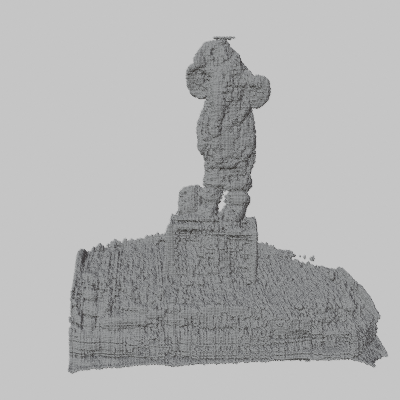
\includegraphics[width=0.6\textwidth]{tensorf-elephant.png}
        \caption{После настройки}
        \label{fig:tensorf_eleph}
    \end{subfigure}
    \caption{Влияние настройки \texttt{scene\_bbox} и \texttt{near\_far}.}
\end{figure}

Чтобы учесть истинные габариты сцены, границы коробки были
расширены до $[-2,2]^3$. Дополнительно изменён диапазон
$\verb|near_far|$ c $[0.1,100]$ до $[1.0,6.0]$.
Параметр \texttt{near\_far} задаёт ближнюю и дальнюю плоскости
отсечения, внутри которых происходит интегрирование вдоль лучей.
Сужая диапазон, мы исключили участок пола, расположенный
за объектом.

После внесения правок и запуска оптимизации на 5000 итераций\footnote{В
контексте TensoRF «итерация» — это один шаг стохастического градиентного спуска,
в котором мини‑батч лучей используется для обновления параметров тензорных
решёток.} за 40 минут метрика PSNR на валидационных изображениях достигла $34.7$ дБ, а
результирующая трёхмерная модель (рис.~\ref{fig:tensorf_eleph})
приобрела чёткий силуэт без шумов и обрезанных частей. Таким образом, даже без
масок TensoRF способен реконструировать объект из реального видео, если
предварительно корректно задать габариты сцены и границы интегрирования по лучу.
